\documentclass{sigchi}

% Use this command to override the default ACM copyright statement
% (e.g. for preprints).  Consult the conference website for the
% camera-ready copyright statement.


%% EXAMPLE BEGIN -- HOW TO OVERRIDE THE DEFAULT COPYRIGHT STRIP -- (July 22, 2013 - Paul Baumann)
% \toappear{Permission to make digital or hard copies of all or part of this work for personal or classroom use is      granted without fee provided that copies are not made or distributed for profit or commercial advantage and that copies bear this notice and the full citation on the first page. Copyrights for components of this work owned by others than ACM must be honored. Abstracting with credit is permitted. To copy otherwise, or republish, to post on servers or to redistribute to lists, requires prior specific permission and/or a fee. Request permissions from permissions@acm.org. \\
% {\emph{CHI'14}}, April 26--May 1, 2014, Toronto, Canada. \\
% Copyright \copyright~2014 ACM ISBN/14/04...\$15.00. \\
% DOI string from ACM form confirmation}
%% EXAMPLE END -- HOW TO OVERRIDE THE DEFAULT COPYRIGHT STRIP -- (July 22, 2013 - Paul Baumann)


% Arabic page numbers for submission.  Remove this line to eliminate
% page numbers for the camera ready copy

%\pagenumbering{arabic}

% Load basic packages
\usepackage{balance}  % to better equalize the last page
\usepackage{graphics} % for EPS, load graphicx instead
%\usepackage[T1]{fontenc}
\usepackage{txfonts}
\usepackage{times}    % comment if you want LaTeX's default font
\usepackage[pdftex]{hyperref}
% \usepackage{url}      % llt: nicely formatted URLs
\usepackage{color}
\usepackage{textcomp}
\usepackage{booktabs}
\usepackage{ccicons}
\usepackage{color,soul}
\usepackage{listings}

% llt: Define a global style for URLs, rather that the default one
\makeatletter
\def\url@leostyle{%
  \@ifundefined{selectfont}{\def\UrlFont{\sf}}{\def\UrlFont{\small\bf\ttfamily}}}
\makeatother
\urlstyle{leo}

% To make various LaTeX processors do the right thing with page size.
\def\pprw{8.5in}
\def\pprh{11in}
\special{papersize=\pprw,\pprh}
\setlength{\paperwidth}{\pprw}
\setlength{\paperheight}{\pprh}
\setlength{\pdfpagewidth}{\pprw}
\setlength{\pdfpageheight}{\pprh}

% Make sure hyperref comes last of your loaded packages, to give it a
% fighting chance of not being over-written, since its job is to
% redefine many LaTeX commands.
\definecolor{linkColor}{RGB}{6,125,233}
\hypersetup{%
  pdftitle={SIGCHI Conference Proceedings Format},
  pdfauthor={LaTeX},
  pdfkeywords={SIGCHI, proceedings, archival format},
  bookmarksnumbered,
  pdfstartview={FitH},
  colorlinks,
  citecolor=black,
  filecolor=black,
  linkcolor=black,
  urlcolor=linkColor,
  breaklinks=true,
}

% create a shortcut to typeset table headings
% \newcommand\tabhead[1]{\small\textbf{#1}}

% End of preamble. Here it comes the document.
\begin{document}

\title{EyeJS: A Framework for Generic Eye-Tracking Interactivity for Web Browsers and Node.JS}

\numberofauthors{2}
\author{%
  \alignauthor{Joshua R. Toenyes\\
    \affaddr{Dept. of Computer Science and Engineering}\\
    \affaddr{University of California San Diego}\\
    \affaddr{La Jolla, California, USA}\\
    \email{joshua.r.toenyes@jacobs.ucsd.edu}}\\
  \alignauthor{Nadir Weibel\\
    \affaddr{Dept. of Computer Science and Engineering}\\
    \affaddr{University of California San Diego}\\
    \affaddr{La Jolla, California, USA}\\
    \email{weibel@ucsd.edu}}\\
}

\maketitle



\begin{abstract}
  150 words...
\end{abstract}



\keywords{eye tracking; eye events; gaze interaction; blink interaction}



\category{H.5.2}{User Interfaces}{Input devices and strategies,
    Interaction styles (gaze and blinks), Screen design}
\category{H.5.4}{Hypertext/Hypermedia}{Architectures, Navigation}



\section{Introduction}
There is an explosion occurring all around us of sensing and computer input devices. Consumer touch screens, webcams, pose recognition \hl{Kinect}, sensing pens \hl{pens?}, \hl{leap motion}, and eye trackers are all relatively new devices to the consumer world, used to gather input from a device user. New patterns of interacting with computers are growing quickly, and are being rapidly adopted by users at large. User gaze is an inevitable input, and is already being used in systems such as automobile attention measurement systems \hl{reference}, and as a generic input device for computers replacing traditional devices such as the mouse \hl{reference}.

Inexpensive remote eye-tracking devices are now becoming available. Tracking hardware will soon be ready for consumers with an array of available software to utilize this new dimension of user input. In the near future we are likely to see eye tracking built-in to user devices \hl{Tobii reference}, and perhaps eye-tracking will become as ubiquitous as the touchscreen. 

More urgent than as an input device for standard users however, eye tracking can be used for people with disabilities to completely replace the mouse and keyboard. On-screen eye typing keyboards \hl{ref} and operating systems designed specifically for use with eyes may soon be available for many more individuals with disabilities as eye tracker become less expensive and more available. Individuals who suffer from paralysis or Locked in Syndrome (LIS) \hl{reference} could soon be nearly as efficient using a computer as someone using a traditional keyboard and mouse.

EyeJS is a framework which endeavors to bring eye-interactivity and
eye-tracking data to the web browser and Node.JS using a low-cost eye
tracker device. 

...

While eye tracking may indeed be a useful input device, it is also equally a an important form of implicit user input. It has been shown that user attention can be measured using eye tracking \hl{ref}.

...

We present EyeJS, a framework ...



There is still a long road ahead for eye tracker device manufacturers and software developers however, and there remains significant improvements to be made in accuracy and techniques to utilize this data in everyday tasks.



Low-cost eye tracking is still not perfect and there remains significant room for improvement. However, if web designers and developers are to remain current, we need to start thinking about how these devices will be used to interact with our websites and web applications in the near future. Similarly, browser vendors should start seriously considering native support for these input devices.

Naturally, our eyes are used as a sensory devices. Things in the world don't normally move or react as a result of us gazing at them. We use our eyes to gather information about our surroundings and hands or other more mechanical means as tools to manipulate our surroundings. So on a fundamental level, we can see why using our eyes to control something is inherently unnatural. \hl{Reference to support this.}

While eye control may seem unnatural and may not be the preferred primary form of input, there are many opportunities to use it .... Nevertheless, there are some users who lack the capability to 

Suppose we were given access to gaze information, in addition to mouse events and keyboard events? Suppose we stopped trying to replicate the mouse experience with gaze information, and accepted that gaze and mouse inputs are inherently different? What could we accomplish given this additional information? How could we build websites and web applications to take advantage of this information? Could we build interfaces that are entirely intent driven, instead of mechanically driven?

The goal of EyeJS is threefold: first to enable generic web navigation on existing websites using low-cost consumer grade eye trackers, second to contribute to the discussion of possible future standardization of web browser eye events, and third to give web developers access to eye events (for users with eye trackers) to enable the use of eye trackers in web apps and Node.JS based desktop application.

... We developed the framework using two eye trackers, Tobii's EyeX
tracker and The Eye Tribe's same-named eye tracker.



\section{Related Work}

Wassermann, Hardt and Zimmermann recognized the analogous relationship between eye and mouse events in the DOM and implemented a framework similar to EyeJS. They defined the layered eye-tracker, websocket and browser-library layered approach, and defined \emph{gaze} events analogous to mouse events, but stopped short of translating those gaze events to mouse events and did not deliver a user evaluation of its effectiveness. Additionally, their system was implemented using high accuracy \hl{(?)} research grade eye trackers which are not available inexpensively to the consumer market.




\hl{Generic Gaze Interaction Events for Web Browsers info...}

\hl{Other references from the above paper, Midas touch, etc.}



\section{Background}
Prior to the development of EyeJS there was no open-source way for web developers to gain access to eye events or user gaze position from the web environment.

We want access to where the user is looking for research tasks, inferring attention \hl{reference about eye as indicator of attention}, and perhaps measuring user engagement.

Some users could use it as an form of input... specifically paraplegics and in the extreme case LIS patients.



\section{EyeJS DOM Events}
EyeJS provides a number of DOM events which may be listened-for in the same manner as a native DOM event (such as \textit{mouseover}, \textit{mousemove}, \textit{mouseout}, etc.). All EyeJS events "bubble up" from the source DOM Element and behave identically to the native events adhering to the W3C's DOM Level 2 Events Recommendation \cite{domlevel1, domlevel2}, so an event listener attached to some element will be called if the corresponding event is triggered on the element itself or any of its children (this is the default behavior of native events \hl{[check if this isn't true for any events]}). Eye events provided by EyeJS are described below.

\subsection{\textbf{\textit{gaze}} Event}
The \textit{gaze} event is fired whenever the user's gaze is over some element. This event is most analogous to a \textit{mousemove} event. Like a \textit{mousemove}, the user may actually be unaware of the element over-which the event is triggered. For example, if the user's eyes are currently executing a saccade while simultaneously being sampled by the eye-tracker, the user will be unaware of the element they are gazing at. \hl{[Lots of references about saccades and unawareness.]} For this reason the \textit{fixation} event is provided (see below).

\subsection{\textbf{\textit{gazeleave}} Event}
The \textit{gazeleave} event is fired on an element whenever the user's gaze transitions from the target element (the one firing the \textit{gazeleave}) to another element. The event is analogous to a \textit{mouseleave}.

\subsection{\textbf{\textit{fixation}} Event}
This event occurs when the user's gaze has remained fixated on a single element for at least 110 milliseconds \hl{[citation about longest saccade duration]}. Since the sample rate of eye trackers can vary, we require consecutive samples of the gaze remaining over a particular element for at least 110 milliseconds to trigger this event. Using this timing we are reasonably sure the user is consciously aware of the element they are gazing at, and that the series of sample eye-tracker sample points were not taken during a saccade. (Assuming the element is of reasonable size of course, as an element the size of the entire screen would constantly trigger a \textit{fixation} event regardless of the movement of their gaze.)

\begin{figure}
\centering
  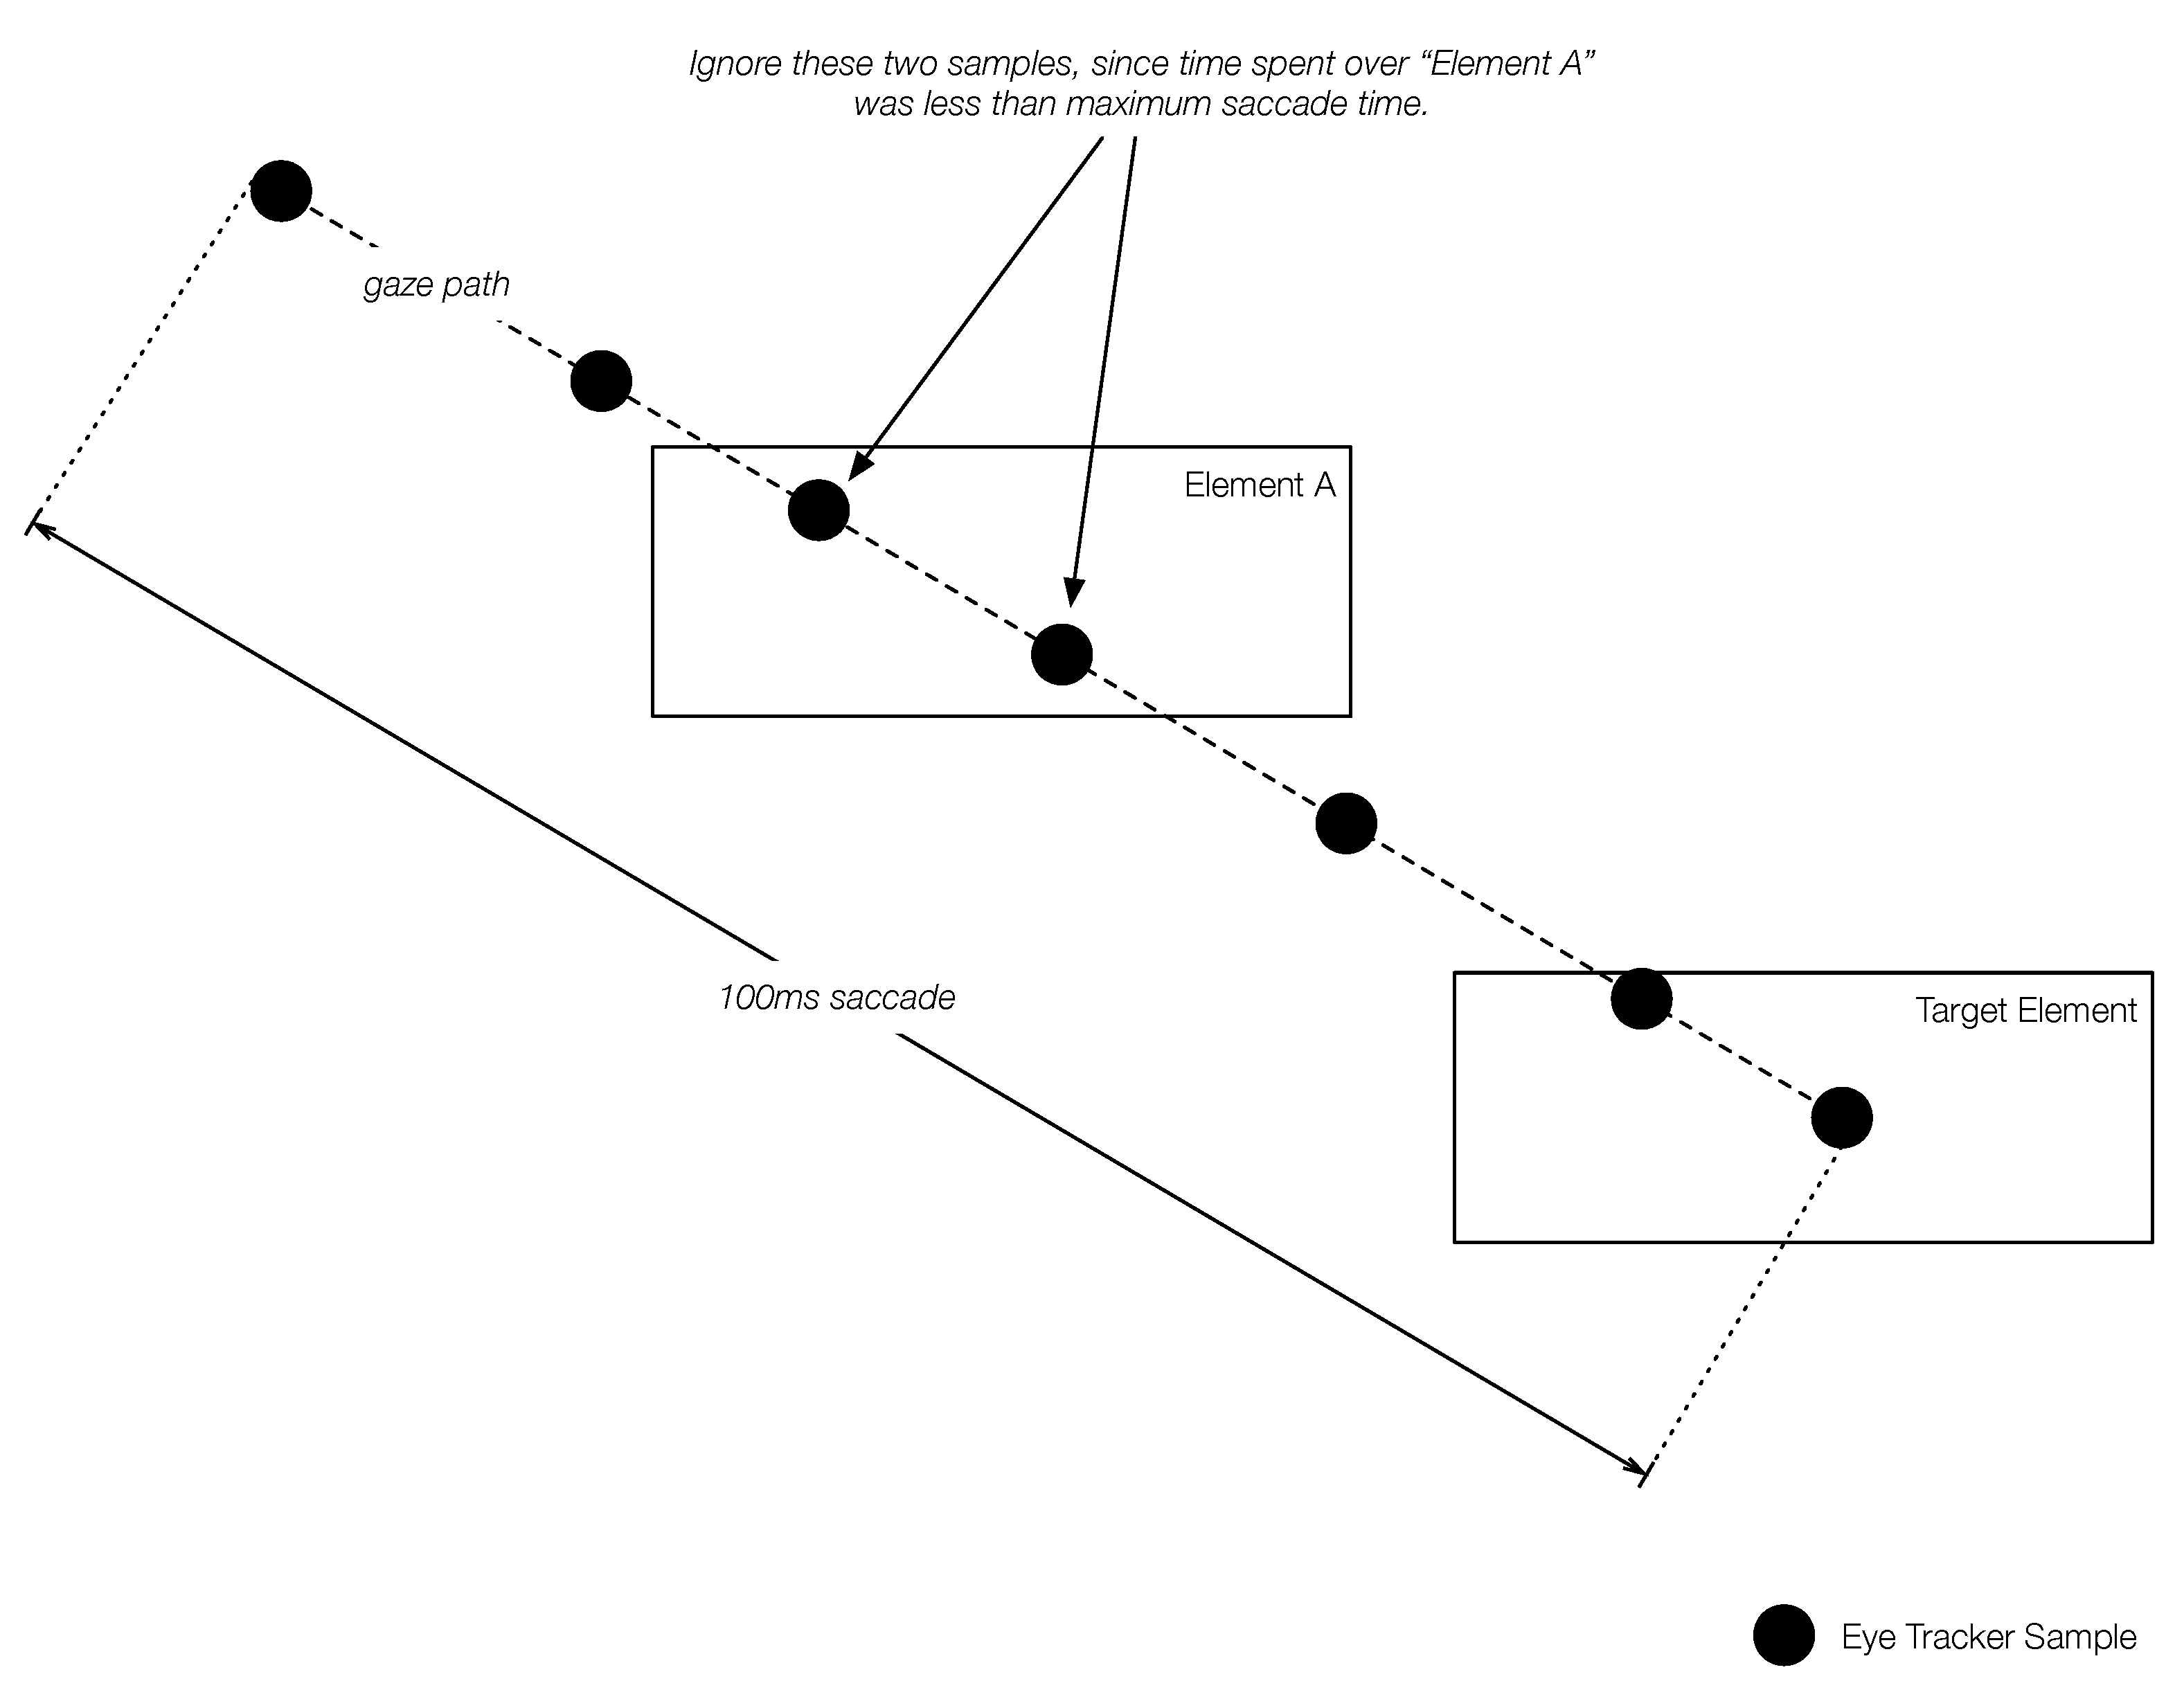
\includegraphics[width=0.9\columnwidth]{figures/saccade.pdf}
  \caption{Eye saccade quickly moving over Element A and fixating on Target Element.}~\label{fig:saccade}
\end{figure}

\subsection{\textbf{\textit{fixationend}} Event}
The \textit{fixationend} event is triggered on an element when the user's gaze transitions away from the subject element. This event is similar to the \textit{gazeleave} event (and indeed a \textit{gazeleave} event is triggered in tandem with a \textit{fixationend}), however it is only triggered when a full fixation occurred prior to the user's gaze departing the subject element.

\subsection{\textbf{\textit{blink}} Event}
Eyes opening and closing is a constant reality of human beings. We constantly blink, but usually quiet quickly. The purpose of the \textit{blink} event is to detect a purposeful and conscious blink. In the author's [opinion?] this was best achieved by timing a blink to be longer than an unconscious blink, but not long enough to be triggered by the eyes leaving the tracker's field of view. \hl{insert sentence about blink timing here.} Using this event, complete hands-free use of the web-browser is possible.

\subsection{\textbf{\textit{eyesopen}} Event}
The \textit{eyesopen} event is triggered whenever both eyes transition from being untracked (or unavailable) to the eye tracker, to both being tracked (or available).

\subsection{\textbf{\textit{eyesclose}} Event}
Similar to the \textit{eyesopen} event, the \textit{eyesclose} event is triggered when both eyes transition from being open to closed, as measured by their tracking availability by the eye-tracker device.



\section{EyeJS Framework Components}
The EyeJS Framework is composed of three layers: first an interface with an eye-tracking device, second a WebSocket server \cite{websocket} which provides raw gaze and eye availability status data in a standardized format on a known local port, and finally a JavaScript library for processing the eye-tracking data and translating it into meaningful events in the web document's Document Object Model (DOM) \cite{domlevel1, domlevel2}. We also developed a Google Chrome Web Browser extension \cite{chromeextensions} to enable eye-interactivity on all web sites \hl{[HTTPs only?]} by injecting the JavaScript library at page load and simulating mouse events.


\subsection{Eye Tracker Interface}
Eye tracking device manufacturers generally provide some type of SDK or interface for communicating with the device. During the course of development, we experimented with eye trackers from two manufacturers, The Eye Tribe's self named eye tracker and the EyeX tracker from Tobii. Each tracker has their own compatibilities and communication interfaces. The eye tracker interface portion of EyeJS gathers tracker-provided screen x and y gaze coordinates, and eye-availability (wether the eye-tracker is currently tracking both, only the left or right, or neither eyes).


\subsubsection{The Eye Tribe Tracker}
The Eye Tribe tracker is compatible with Windows 7 and 8 and Apple's Mac OS X with Google Android OS support in-development. SDKs are provided in C\#, C++ and Java, and it also has a well documented API for communication via a TCP interface using JSON formatted messages. We opted to develop a JavaScript SDK and Node.JS application to communicate with this device using its TCP API. This allowed all three layers (eye-tracker communication, WebSocket server, and on-page JS library) to all be written in JavaScript. This device provides raw un-smoothed screen gaze coordinates.


\subsubsection{EyeX Tracker}
Tobii's EyeX tracker is only compatible with Windows 7 and 8 and provides SDKs for .NET, C/C++, and Unity. No other type of interface is offered or documented making user-built SDKs in other languages impossible. To communicate with the EyeX device, we developed a lightweight C++ application. The EyeX tracker performs a small amount of smoothing on the screen coordinates prior to providing them in software, although there is an additional SDK available (the Tobii Gaze SDK) which provides access to the raw, un-smoothed data. We did not use this SDK for EyeJS.


\subsection{WebSocket and EyeJS Subprotocol}
After the screen gaze coordinates are collected from the eye-tracker, they must be made available for a web-browser running on the same host. This is accomplished using a WebSocket server which provides lightweight low-latency 2-way communication between the web-browser and the server. The WebSocket server provides an interface running on a known port, 5225 \hl{[check the port]}, which the JavaScript library running on a web-page connects to.

\subsubsection{EyeJS WebSocket Subprotocol}
EyeJS communication currently occurs in only one direction, from the WebSocket server to client web-browsers. We did not implement any eye-tracker commands. The format of these messages are well defined and standardized for both the Tobii EyeX tracker and The Eye Tribe trackers. Conceivably, the EyeJS Framework could be extended to include other eye-trackers, which would only need to provided a WebSocket interface implementing this subprotocol. Each message is formatted as follows:

\begin{lstlisting}
{
  // event type
  type: 'gaze',

  // millisecond timestamp
  timestamp: < number >,

  // mean gaze screen-coordinates of
  // both left and right eyes
  avg: {
    x: < number >,
    y: < number >
  },

  // left-eye gaze screen-coordinates
  // of only left eye
  left: {
    x: < number >,
    y: < number >
  },

  // right-eye gaze screen-coordinates
  // of only left eye
  right: {
    x: < number >,
    y: < number >
  }

  // true if the indicated eye is being
  // tracked by the eye-tracker
  available: {
    left:   < boolean >,
    right:  < boolean >,
    both:   < boolean >
  }
}
\end{lstlisting}


\subsection{EyeJS JavaScript Library}
The JavaScript library processes and converts the eye tracker data into meaningful events within the web-browser.

\subsubsection{Data Smoothing}

\subsubsection{}


\subsection{EyeJS Google Chrome Extension}
To facilitate complete web browsing capability using eye-control, we developed a Google Chrome extension. The extension automatically injects the EyeJS JavaScript library on every page, translate the eye events to mouse events, adds a keypress event to mimic a mouse click, and adds visual eye-interactive controls for navigating forward and backward in the browser history (replicating the forward and back buttons) and scrolling up and down.

\hl{add figure of controls}

The forward and back controls are curved semi-transparent buttons on the left and right sides of the screen which slide in-and-out of view. The scrolling controls slide in-and-out of view in the same fashion and are located on the top and bottom of the screen. To trigger the appearance of any of these controls, the user must only look slightly off the screen edge of the control they wish to appear. For example, if the user wishes to navigate "back" to the previous page, they would look slightly off the left side of the screen which would cause the back control to appear. The user could then activate the control (by clicking-on, blinking, or pressing the control-key while fixated on the element).

The scroll controls work slightly differently, as they are of a continuous nature. Instead of blinking on the scroll controls, as long as the user gazes as the scroll control the page will scroll in the corresponding direction (e.g. to scroll up, the user must only gaze at the "scroll-up" control). Scrolling ceases as soon as the user's gaze leaves the control. To enable quickly scrolling large distances, the scroll speed increases linearly up to some maximum speed proportional to the length of time the user has been looking at the scroll control, that is, the longer the user gazes at the scroll control, the faster the scrolling. \hl{double-check... is it linear?}



\section{Inferring User Intent}
The web is a dynamic place, potentially any DOM element can be interactive. Ideally, anchor tags, buttons, form inputs, and other standardized HTML elements should be used by the user to interact with a website, but nothing prevents the developer from making generic tags such as \textbf{DIV}'s, \textbf{SPAN}'s, or other mostly semantically meaningless tags interact. Indeed in some scenarios it's desirable for these generic tags to be interactive. This presents a challenge for EyeJS however, because we must determine which element the user intends to interact with when using relatively noisy user gaze positions.

What makes this more difficult is that user gaze is inherently non-specific. \hl{Reference about gaze field degrees and what that converts to in pixels.} In contrast, a mouse pointer is accurate to-the-pixel. Since user interfaces are usually developed with the mouse expected to be the primary input device, we must find a way to emulate the pixel perfect accuracy and somehow determine which element the users likely intends to interact with based on the information we have available \hl{go back and define what data we have}. We approach this problem in two steps: first by smoothing and thresholding incoming gaze data, then by using a weighted and biased DOM element selector to determine the element the user likely intends to interact with.


\subsection{Gaze Smoothing}
While incoming eye tracker data can be quiet good, we realized that gaze coordinate smoothing was required. In our experience, even when the user is staring at a simple point, eye-tracker provided gaze coordinates can still vary by \hl{5 to 20?} pixels frame-to-frame in event the best case. To combat this we implemented a simple thresholded exponential smoothing algorithm. Incoming gaze coordinates are run through this algorithm which prevents jitter... \hl{insert specific information about the algorithm and formula}.


\subsection{Element Selection}
After incoming gaze data has been sufficiently smoothed, we need a way to infer which element the user will likely intend to interact with. To do this, we take a series of radial samples around the smoothed gaze center. The element under each point is sampled using the native function \hl{functionName()}. In generic element selection, the element sampled the most times \hl{(the most number of votes?)} will be determined as the interaction candidate. The radial distance between sample points is fixed, as is the angle between radii. This weights the center of the smoothed gaze coordinates higher since there are more sample points per unit area.

\begin{figure}
\centering
  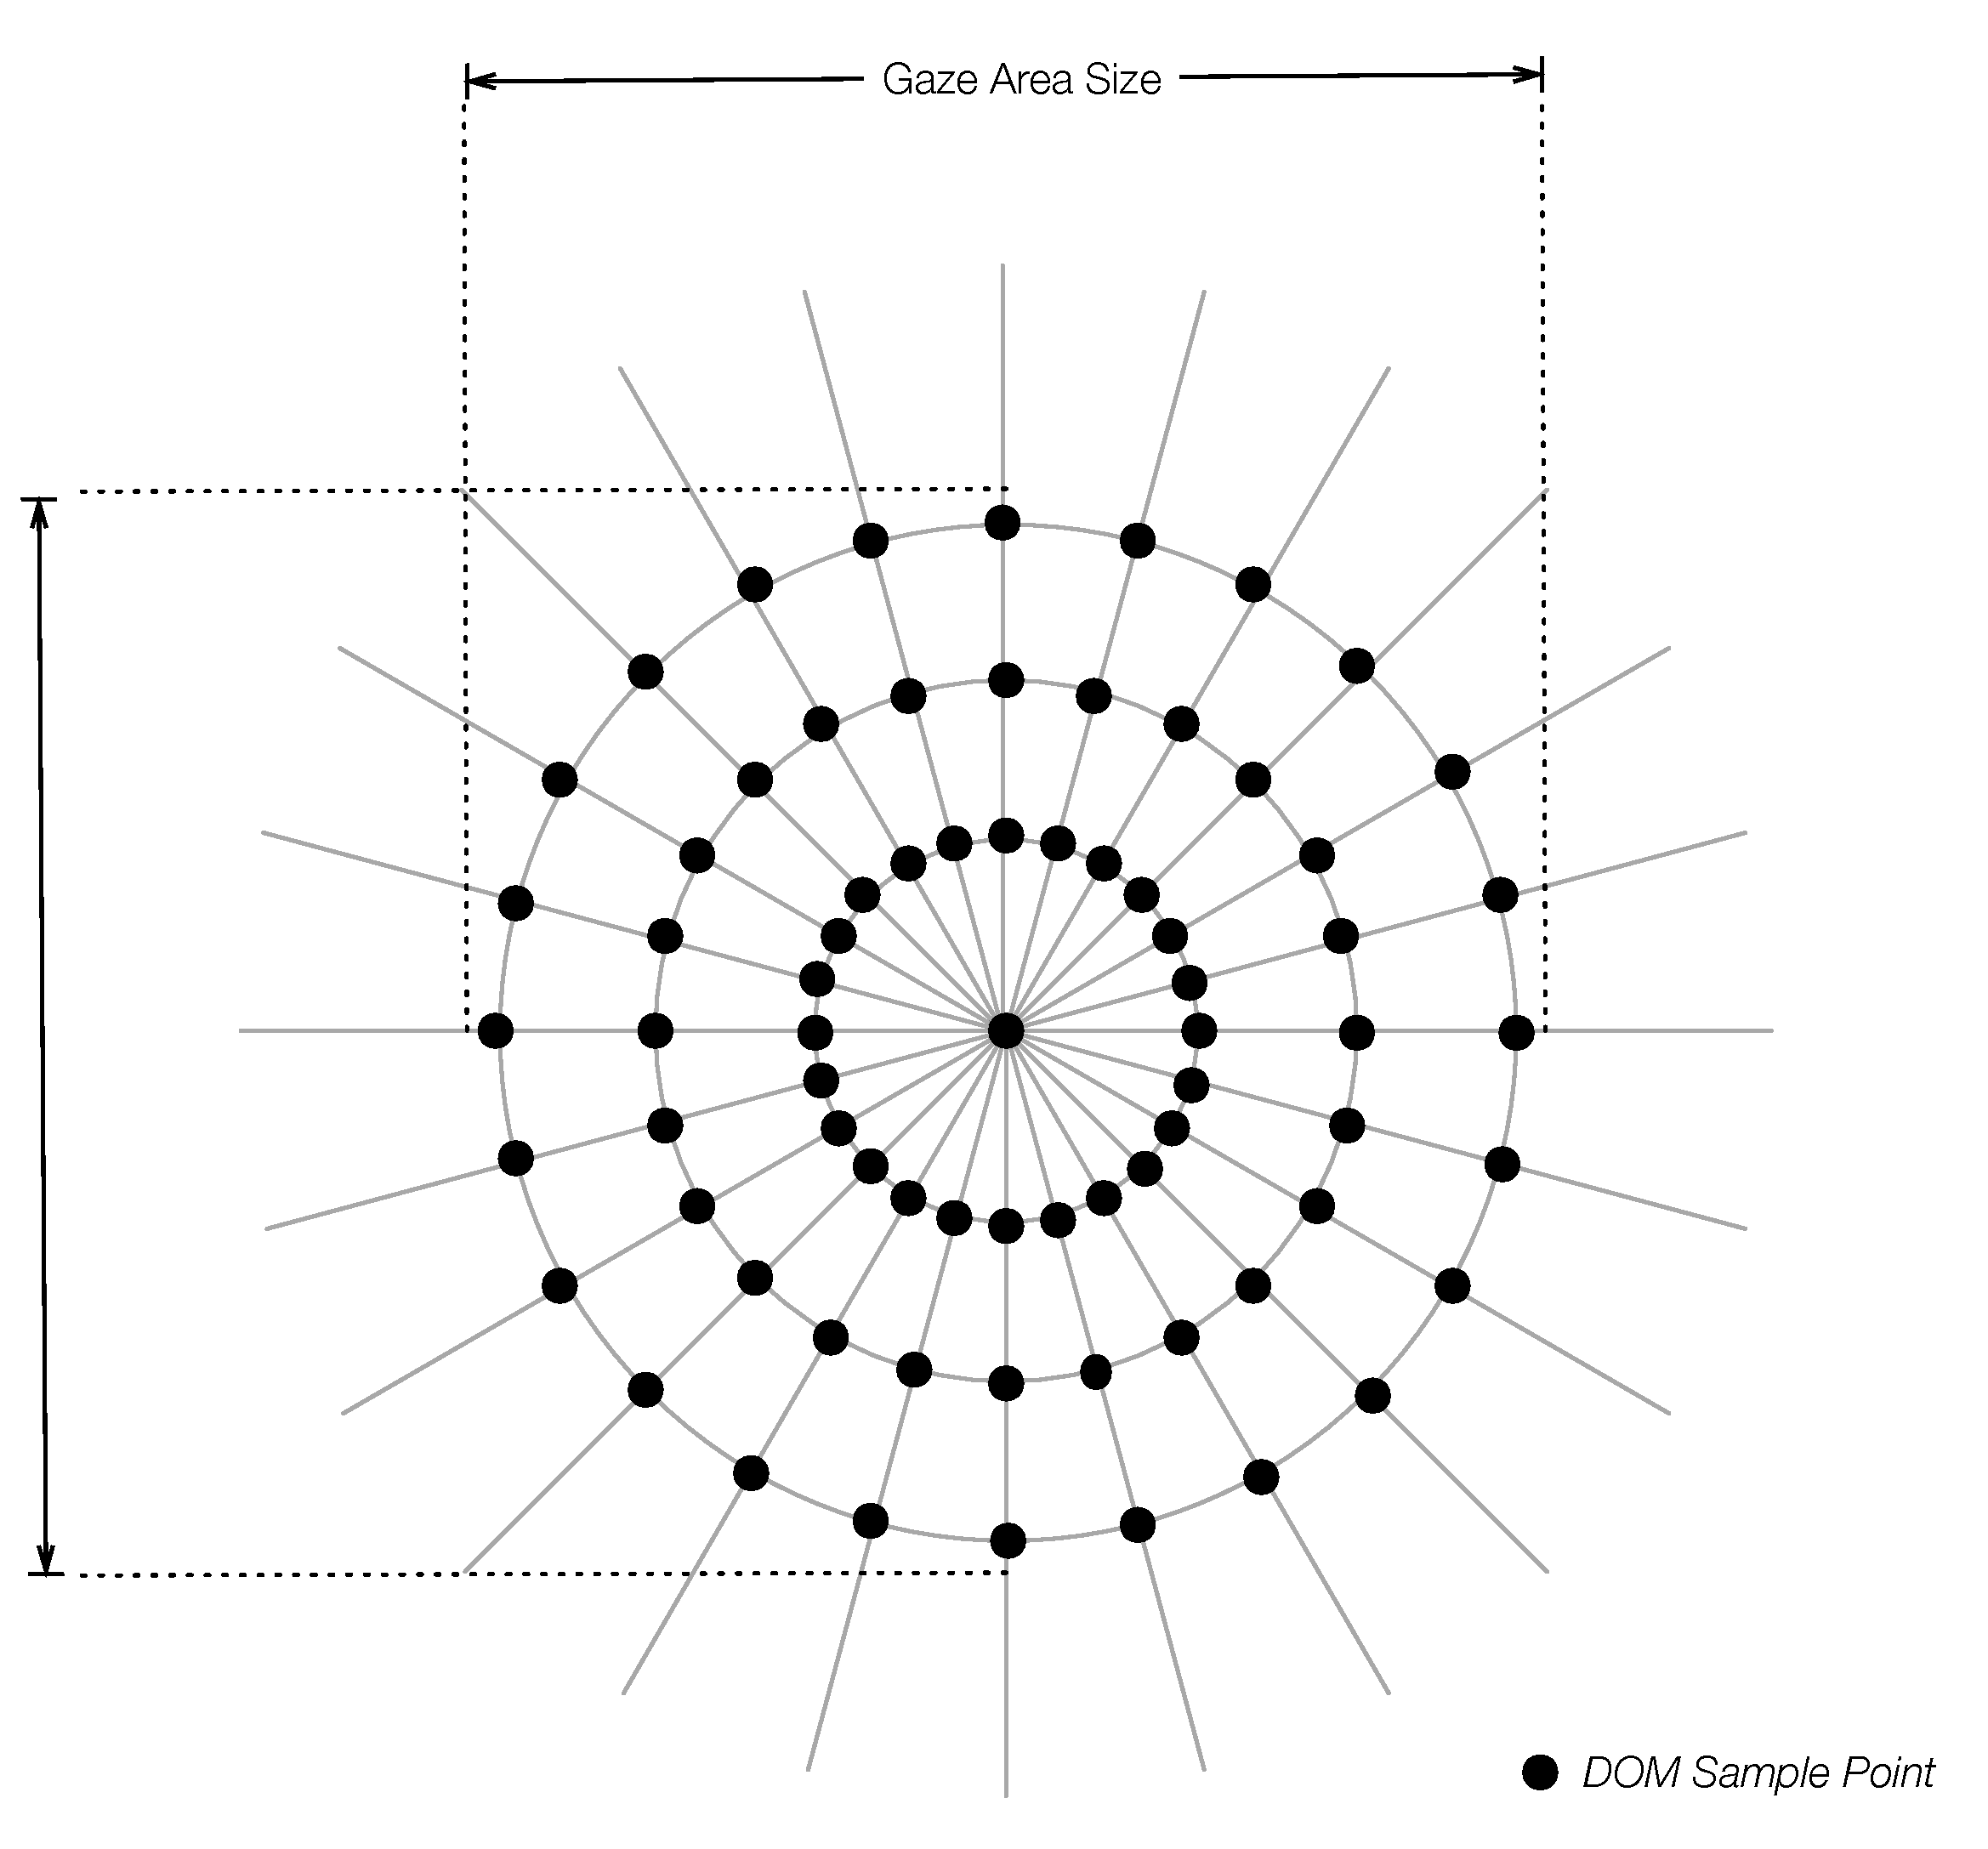
\includegraphics[width=0.9\columnwidth]{figures/dom-sample-points.pdf}
  \caption{DOM sample points are arranged in a radial pattern, 
  naturally giving the gaze center a heavier weight.}~\label{fig:dom-sample-points}
\end{figure}

This voting approach is not always appropriate. For example, if the user's gaze is very close to an anchor element, it's likely they intend to interact with the anchor even though there are more points sampled of the paragraph. Similarly, the developer may wish to "snap" the user's gaze to a particular element if it get's close, thereby making user interaction easier. To accommodate both of these and similar scenarios, we have biased the selection algorithm to strongly prefer specific tags and elements with specific attributes over generic elements. \hl{Insert element precedence and attributes.}

\hl{paragraph and anchor diagram}



\section{Evaluation}
The accuracy and effectiveness of the EyeJS system was tested with \hl{twenty} volunteers, each tasked with completing four experiments, described below. The participants ranged in age from \hl{min-age} to \hl{max-age}, and represented a range of races and computer usage habits. The large majority of participants had never used an eye tracker prior to their participation and none had over 30 minutes of eye tracker usage prior to this trial.

\hl{Insert list of stats about participants including how many had experience using eye trackers.}

We conducted four experiments with each user: a \emph{Simple Navigation Task}, a \emph{Complex Navigation Task}, a \emph{Button Activation Sequence} task, and a \emph{User Focus} task. Each experiment is described in detail below.

\subsection{Evaluation Hardware}
The evaluation was conducted on a Macbook Pro running Windows 7, using a Tobii EyeX eye tracker. The web browser used was Google Chrome, and the Chrome plugin component of EyeJS was installed and running for all experiments. A separate Node.JS application was installed and running to collect and log user data and statistics during the experiments, and a Node.JS-based web server was running as an interface to collect the participants' information, conduct a post-experiment survey, and to act as a web-server for the \emph{button Activation Sequence} task and \emph{User Focus} task.

We choose to use the Tobii EyeX eye tracker to conduct the trials because in our experience developing EyeJS and other applications, it has proved to be more accurate than The Eye Tribe eye tracker. Additionally, the EyeX tracker was more forgiving of user movement during usage. In our experience, The Eye Tribe would require multiple re-calibrations during use to maintain accuracy while the EyeX tracker did not suffer from this inconvenience. We did not however conduct any trials to measure the performance difference between the two. 

The Tobii EyeX tracker was mounted below the laptop screen (as directed by the manufacturer). Users were directed to sit comfortably in front of the laptop and eye tracker was positioned at an appropriate distance as indicated by the eye tracker's calibration utility. 


\subsection{Input Modalities}
Three of the four experiments were accomplished three times (with minor variations each time), once using a trackpad as their primary input, once using EyeJS with keypress activation (the left control-key) to click and select elements, and once using blinks to activate and select elements. The fourth experiment only used the trackpad as an input device. For textual input (i.e. entering information into a search box) the user was directed to select the text-inputs using the current input modality (keypress, blink or click), then enter the information using the keyboard. The order in-which each participant conducted the experiments was randomized, as well as the order of the inputs modalities used to complete the experiments. 

\hl{Supporting information about why the trackpad is a valid comparison.}


\subsection{Experiment Descriptions}
For experiment tasks that required the users to locate specific pieces of information on a web page, the user was verbally directed to its general location on the page, e.g. "left side near the bottom," or "in the grey box half-way down the page." The purpose of this was to prevent experiment completion time measurements from being drastically effected by people unfamiliar with a web site from spending a large portion of time search for the requested information.

\subsubsection{Simple Navigation Task}
This experiment directed the user to perform a series of tasks and navigations on Wikipedia (http://www.wikipedia.org). They were directed to navigate between several pages, perform a search task, and locate information on a given page. Each time the experiment was conducted (once for each input modality) the piece of information to collect changed. Directions for completion of this task were dictated to the participant during the tasks.

\subsubsection{Complex Navigation Task}
This experiment directed users to perform a series of navigation and search tasks on Amazon.com (http://www.amazon.com). Amazon's website is more complex and dynamic than Wikipedia, so the purpose of this experiment was to give the user a more difficult navigation task. Similar to the \textit{Simple Navigation Task}, the tasks of this experiment were dictated to the user.

\subsubsection{Button Activation Sequence}
This experiment presented the user with a sequence of four uppercase letters (the target sequence) and a set of 16 buttons (four rows of four buttons). Each button was labeled with an uppercase letter, four of them having the letters from the sequence. The target sequence, as well as the button labels and their positioning was all randomly generated. As the user completed the selections in the given sequence the buttons would glow red (for incorrect selections), or fade to grey if they were correctly activated (along with the corresponding letter from the target sequence). 

\begin{figure}
\centering
  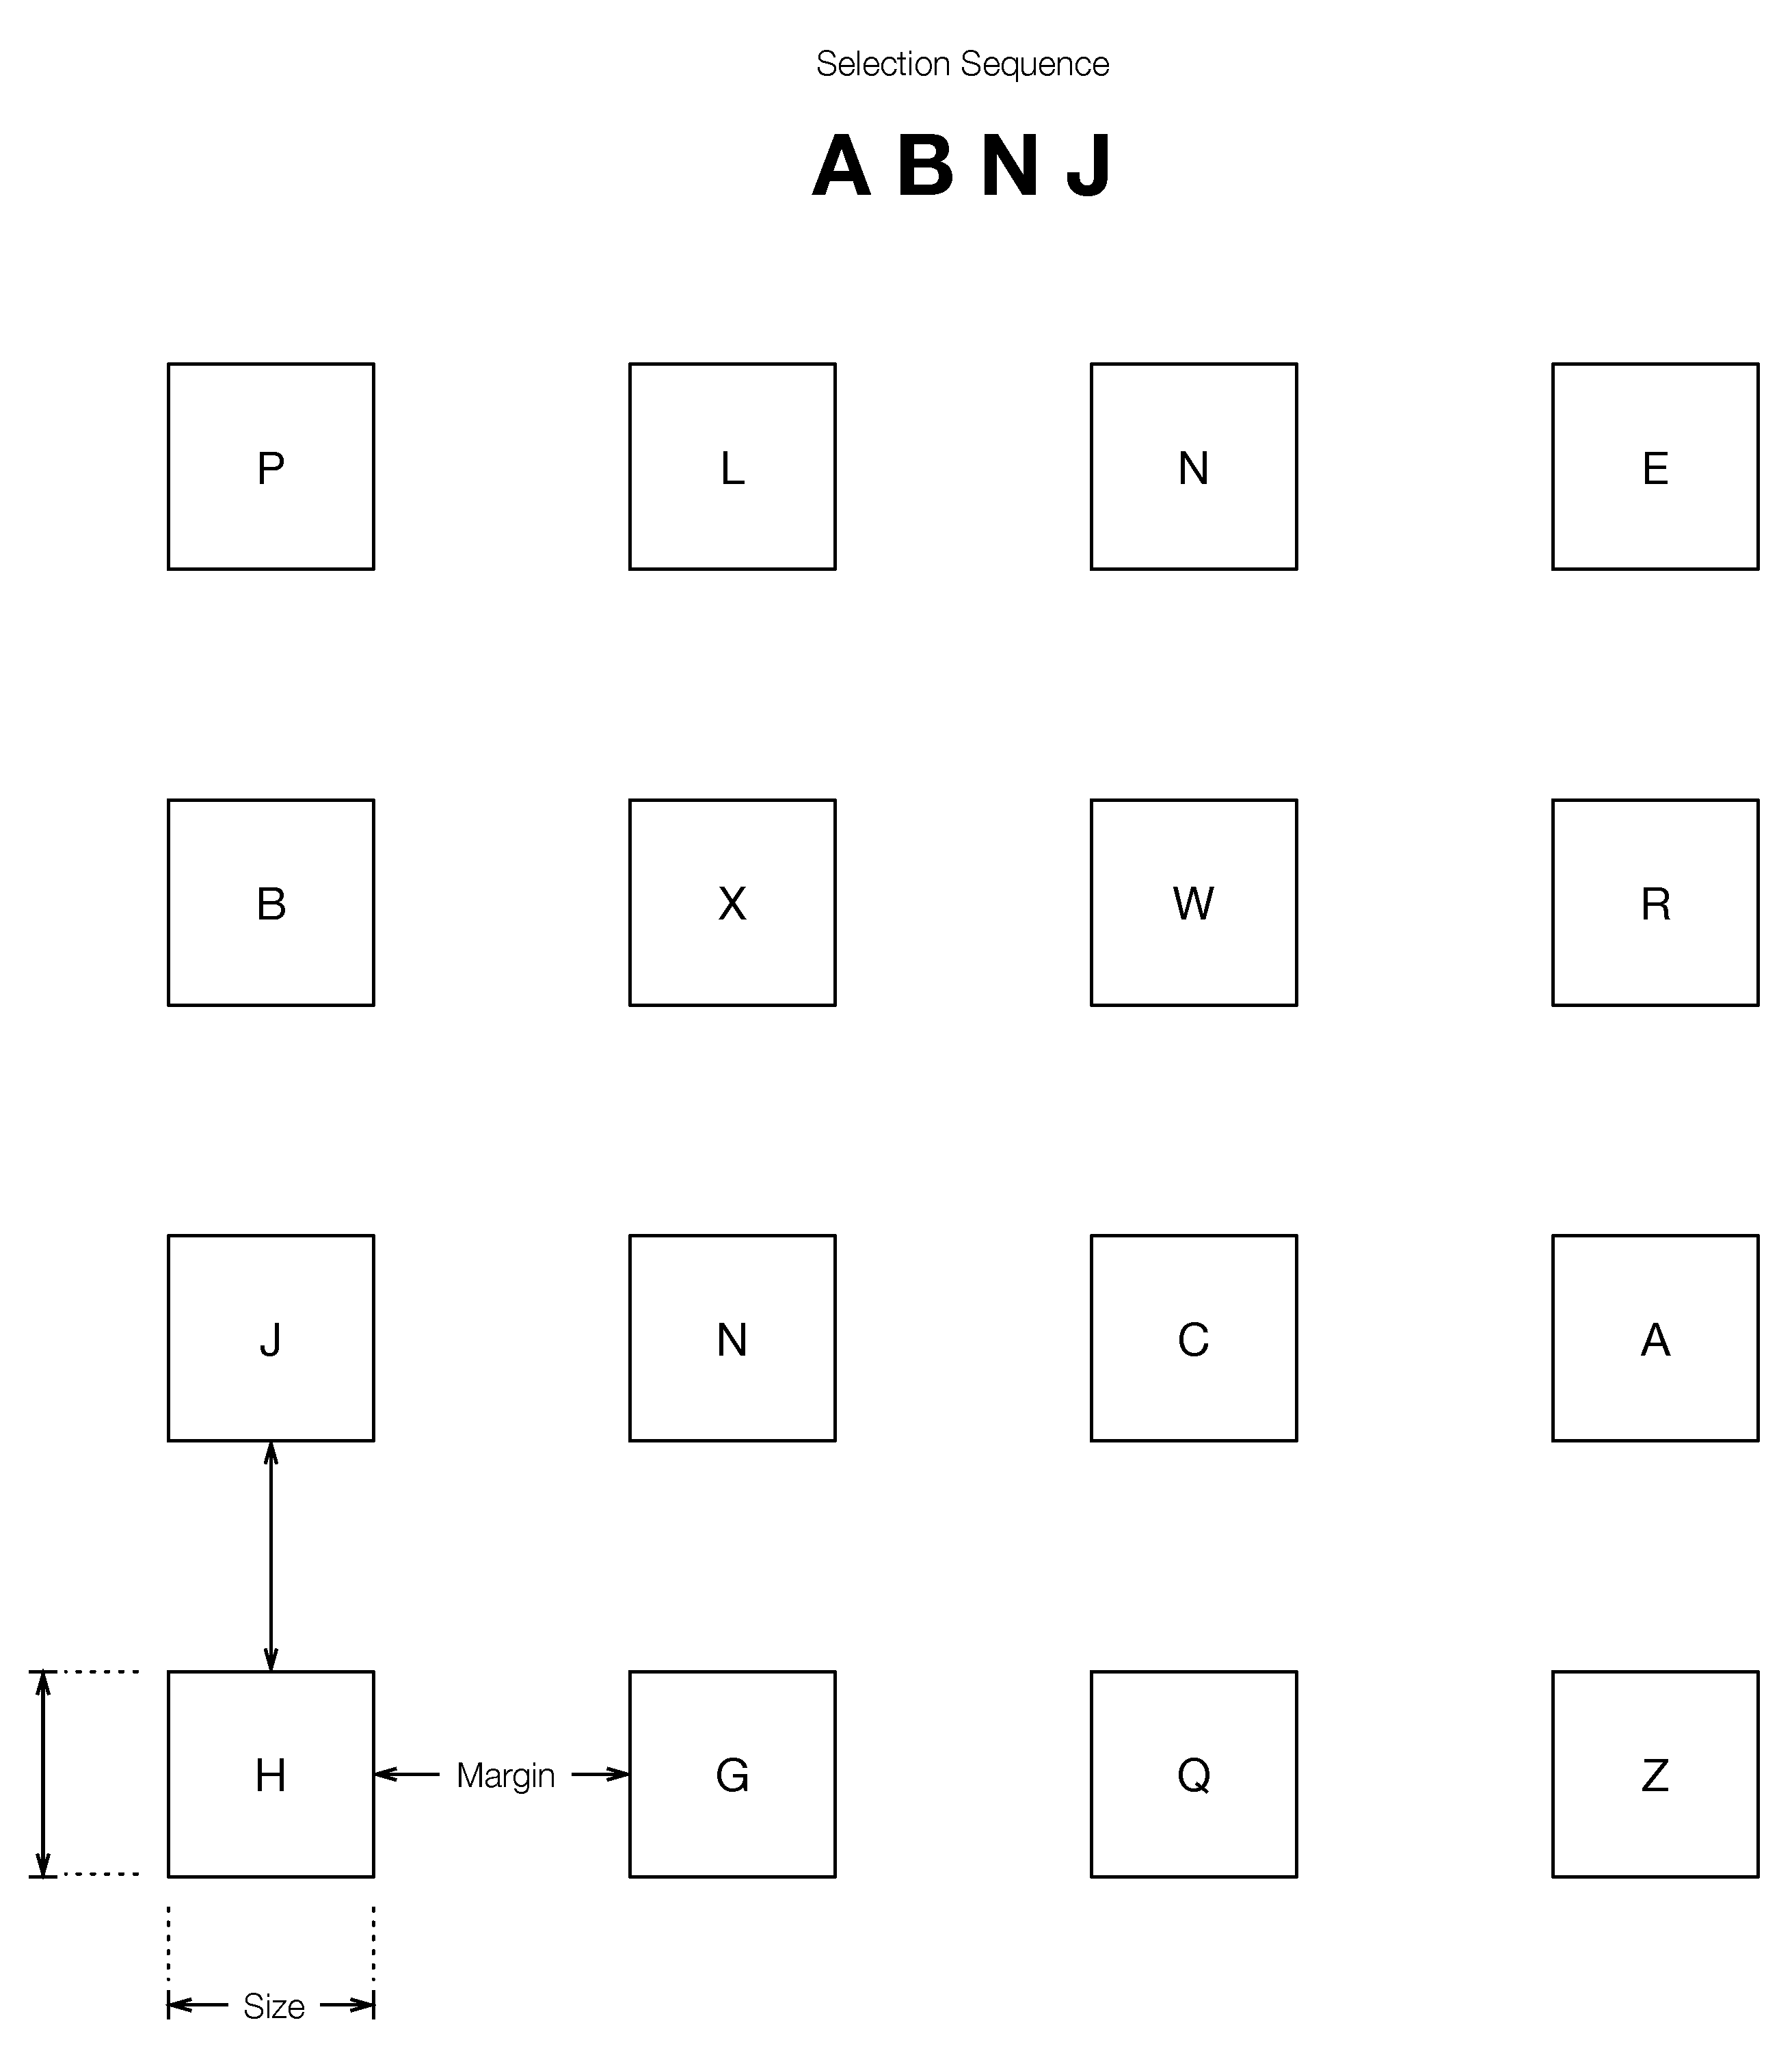
\includegraphics[width=0.9\columnwidth]{figures/sui.pdf}
  \caption{Button activation task with variable button margin sizes.
  }~\label{fig:sui}
\end{figure}

During the course of the experiment, the size of the buttons would shrink, and for each button size, three margin sizes between the buttons would be tested \hl{insert sizes and margin sizes here}. The user's accuracy was continually calculated during the experiment and if they dropped below an accuracy of \hl{insert accuracy}, or took longer than 30 seconds to complete a selection, the experiment for that modality would terminate.

\subsubsection{User Focus}
For this experiment the user was presented with two webpages and directed to complete a Cloze test \hl{insert reference} on the given page. Each page had a sidebar of animated gif's, intended to distract the user. On one page, the animated gif's were faded to approximately 10\% opacity, but would fade-in to 100\% opacity if the user gazed at the sidebar. The intent of the experiment was to determine if the user's focus was affected, and hence task completion time, was affected by the fading effect of the sidebar. In other words, would the user complete the Cloze test faster on a page with a faded distracting content which would fade in to view when looking at it.


\subsection{Results}
The mean trial duration (time it took each participant to complete all the tasks) was \hl{32 minutes}. In general, it took users longer to perform tasks using the eye tracker, for both blink and keypress input modalities, than the trackpad. The keypress input mode was faster than blinks. Figure \ref{fig:task-durations} compares task completion time for experiments which used all three input modalities.

Of the \hl{twenty} participants, \hl{five} had severe difficulties using the system and were unable to complete the experiment tasks. For these users, the eye tracker was unable to provide accurate enough data for the system to be useful. Of these five users, three were wearing very high prescription eyeglasses and were unable to reasonably see the screen without them.

\begin{figure}
\centering
  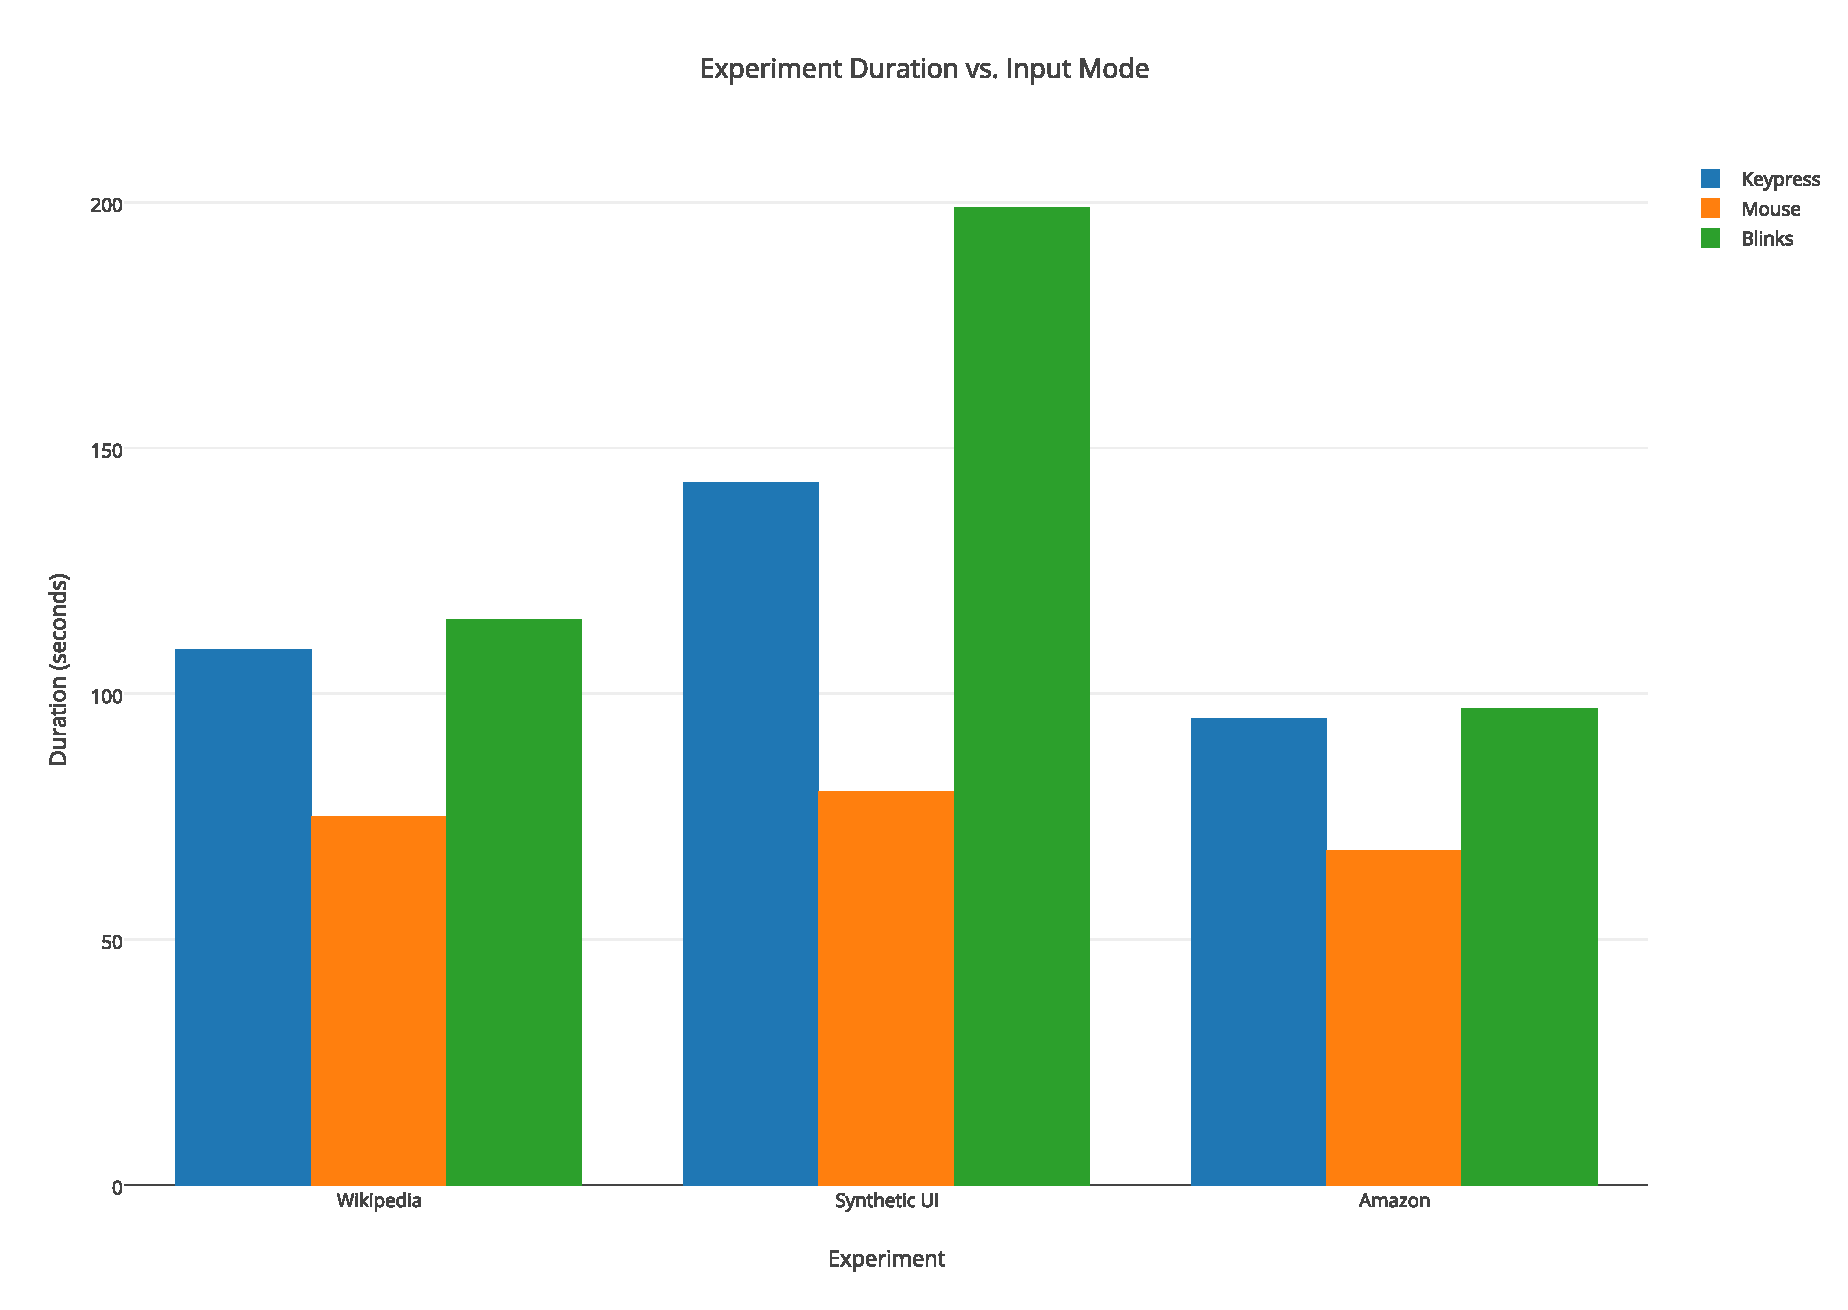
\includegraphics[width=0.9\columnwidth]{figures/task-durations.pdf}
  \caption{Comparison of task duration to input modality.
  }~\label{fig:task-durations}
\end{figure}

\begin{figure}
\centering
  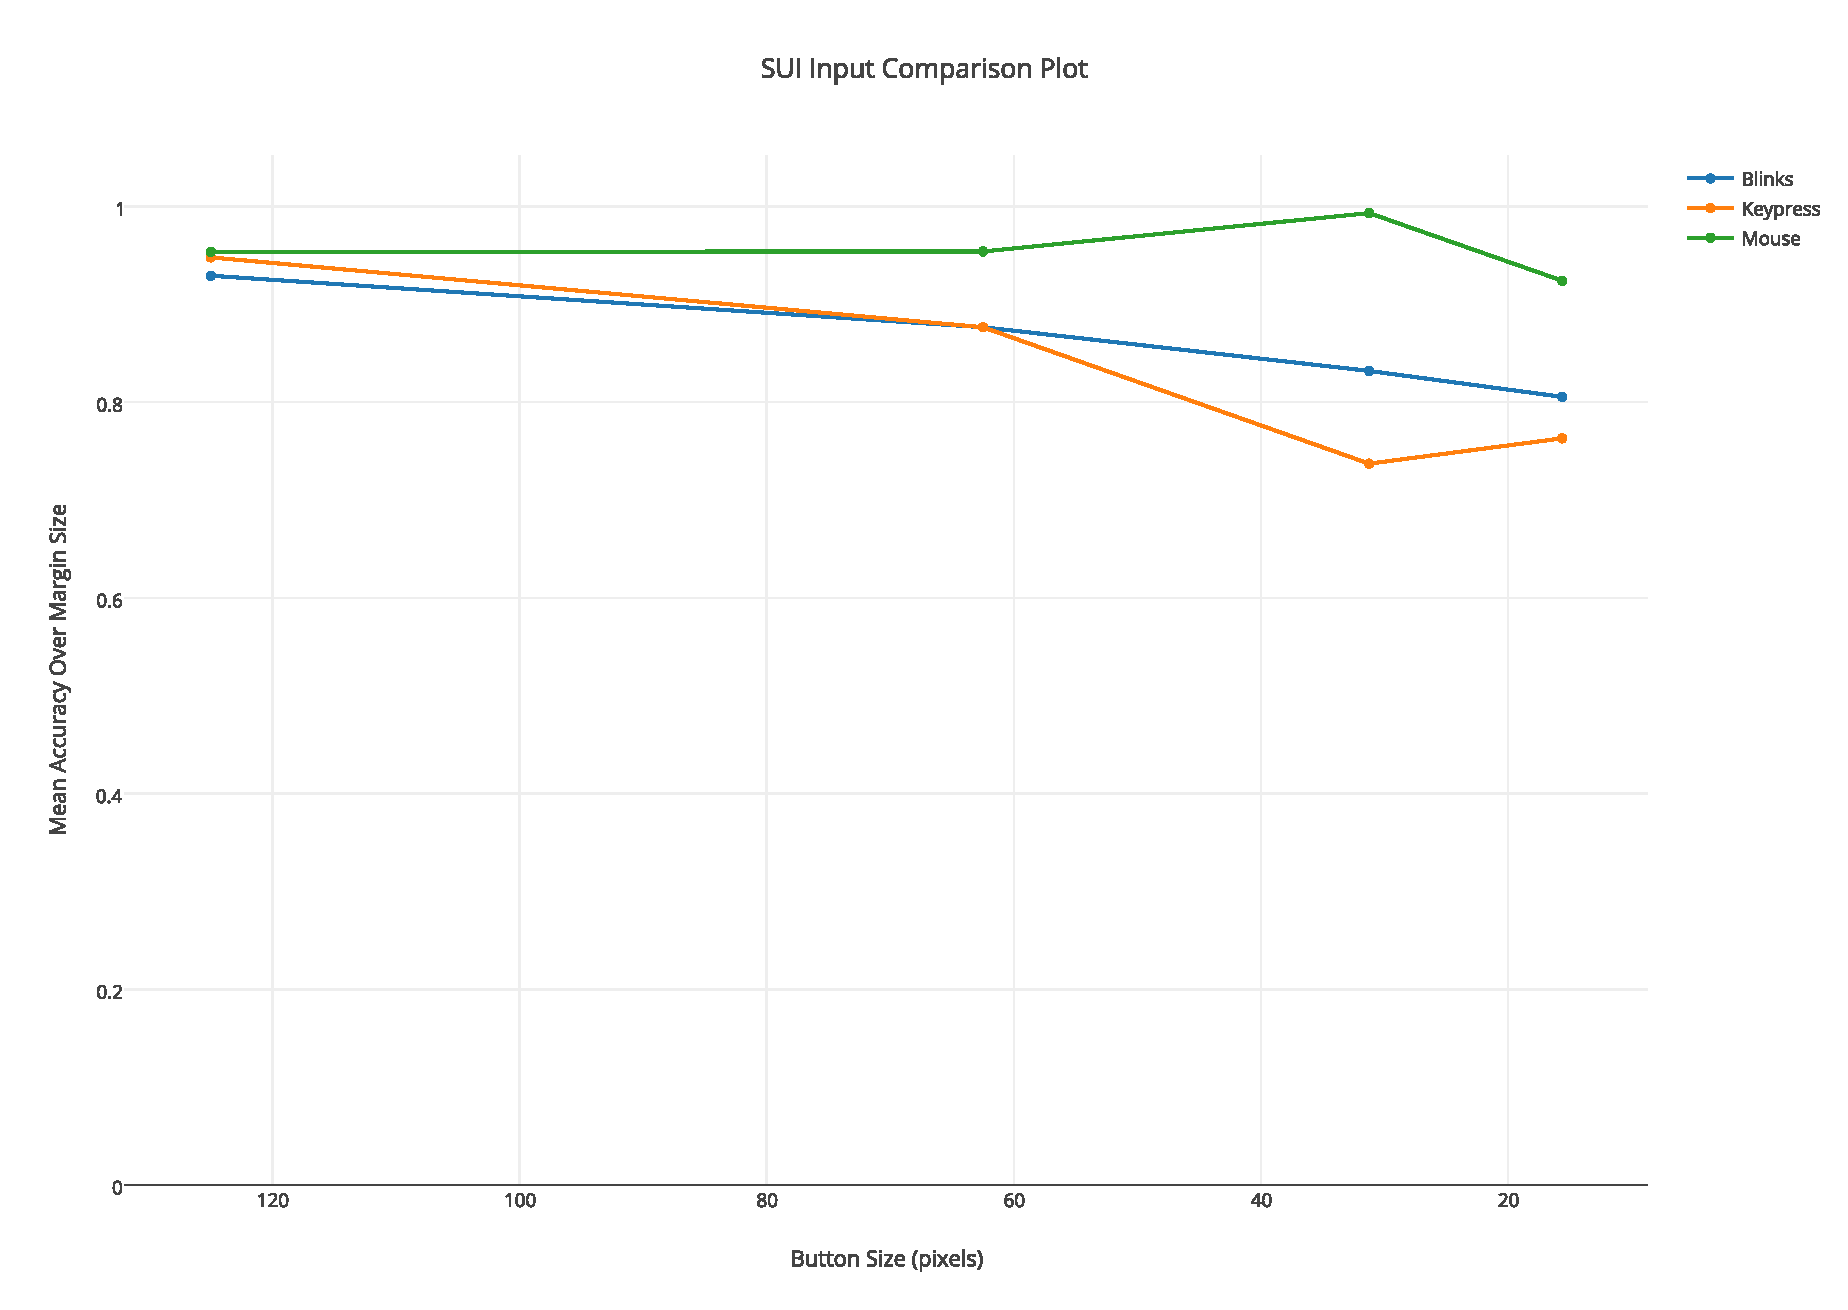
\includegraphics[width=0.9\columnwidth]{figures/mean-accuracy.pdf}
  \caption{Accuracy averaged over margin sizes compared to button size.
  }~\label{fig:mean-accuracy}
\end{figure}

For the \emph{Button Activation Sequence} task, user accuracy was measured and compared across input modalities, button size, and margin size. Eye input accuracy tended to decrease as the size of the buttons decreased while trackpad accuracy remained relatively constant. We can also see that button size had more of an impact on accuracy than the margin between buttons.

\begin{figure}
\centering
  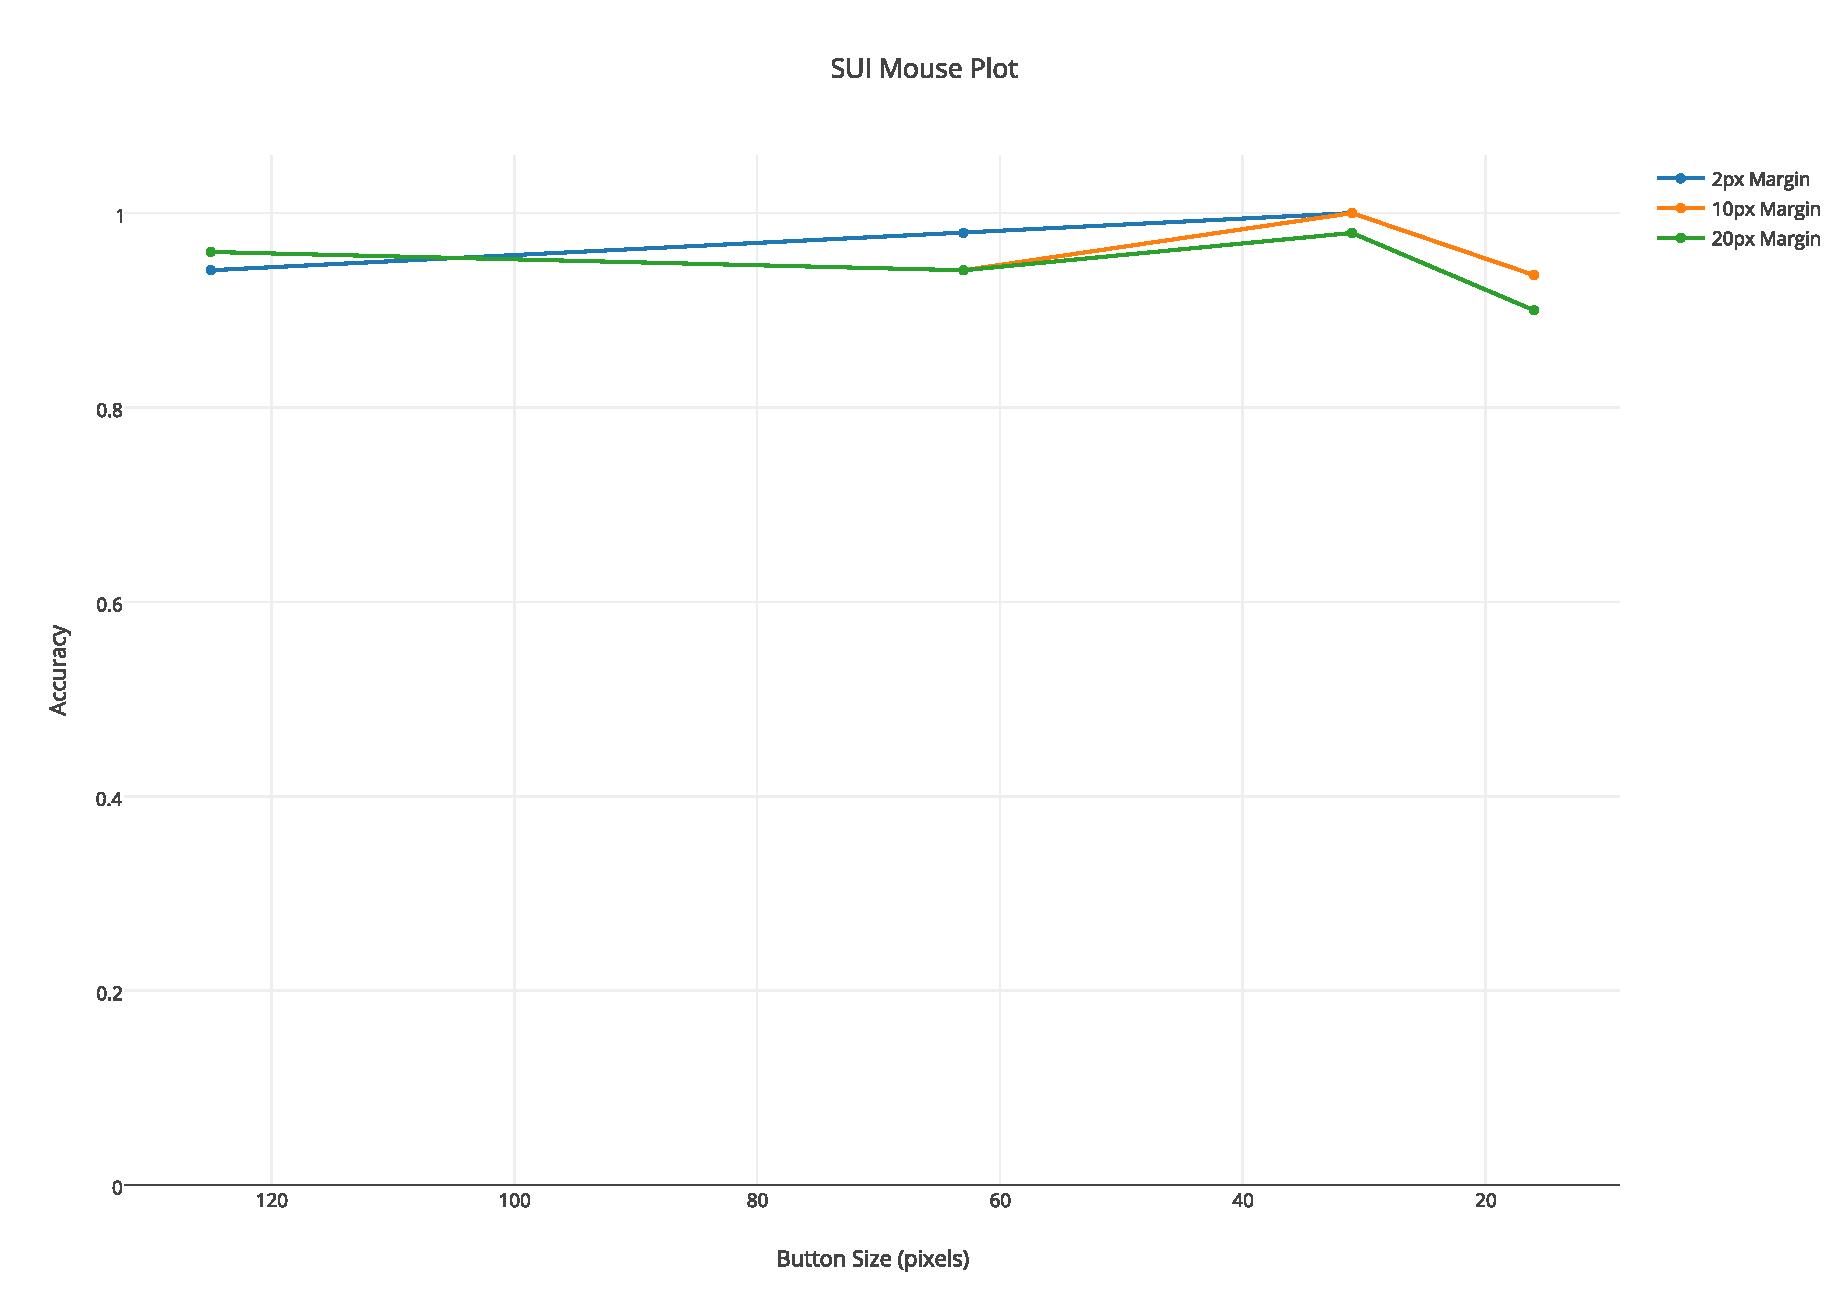
\includegraphics[width=0.9\columnwidth]{figures/mouse-accuracy.pdf}
  \caption{Trackpad accuracy with various margin and button sizes.
  }~\label{fig:mouse-accuracy}
\end{figure}

\begin{figure}
\centering
  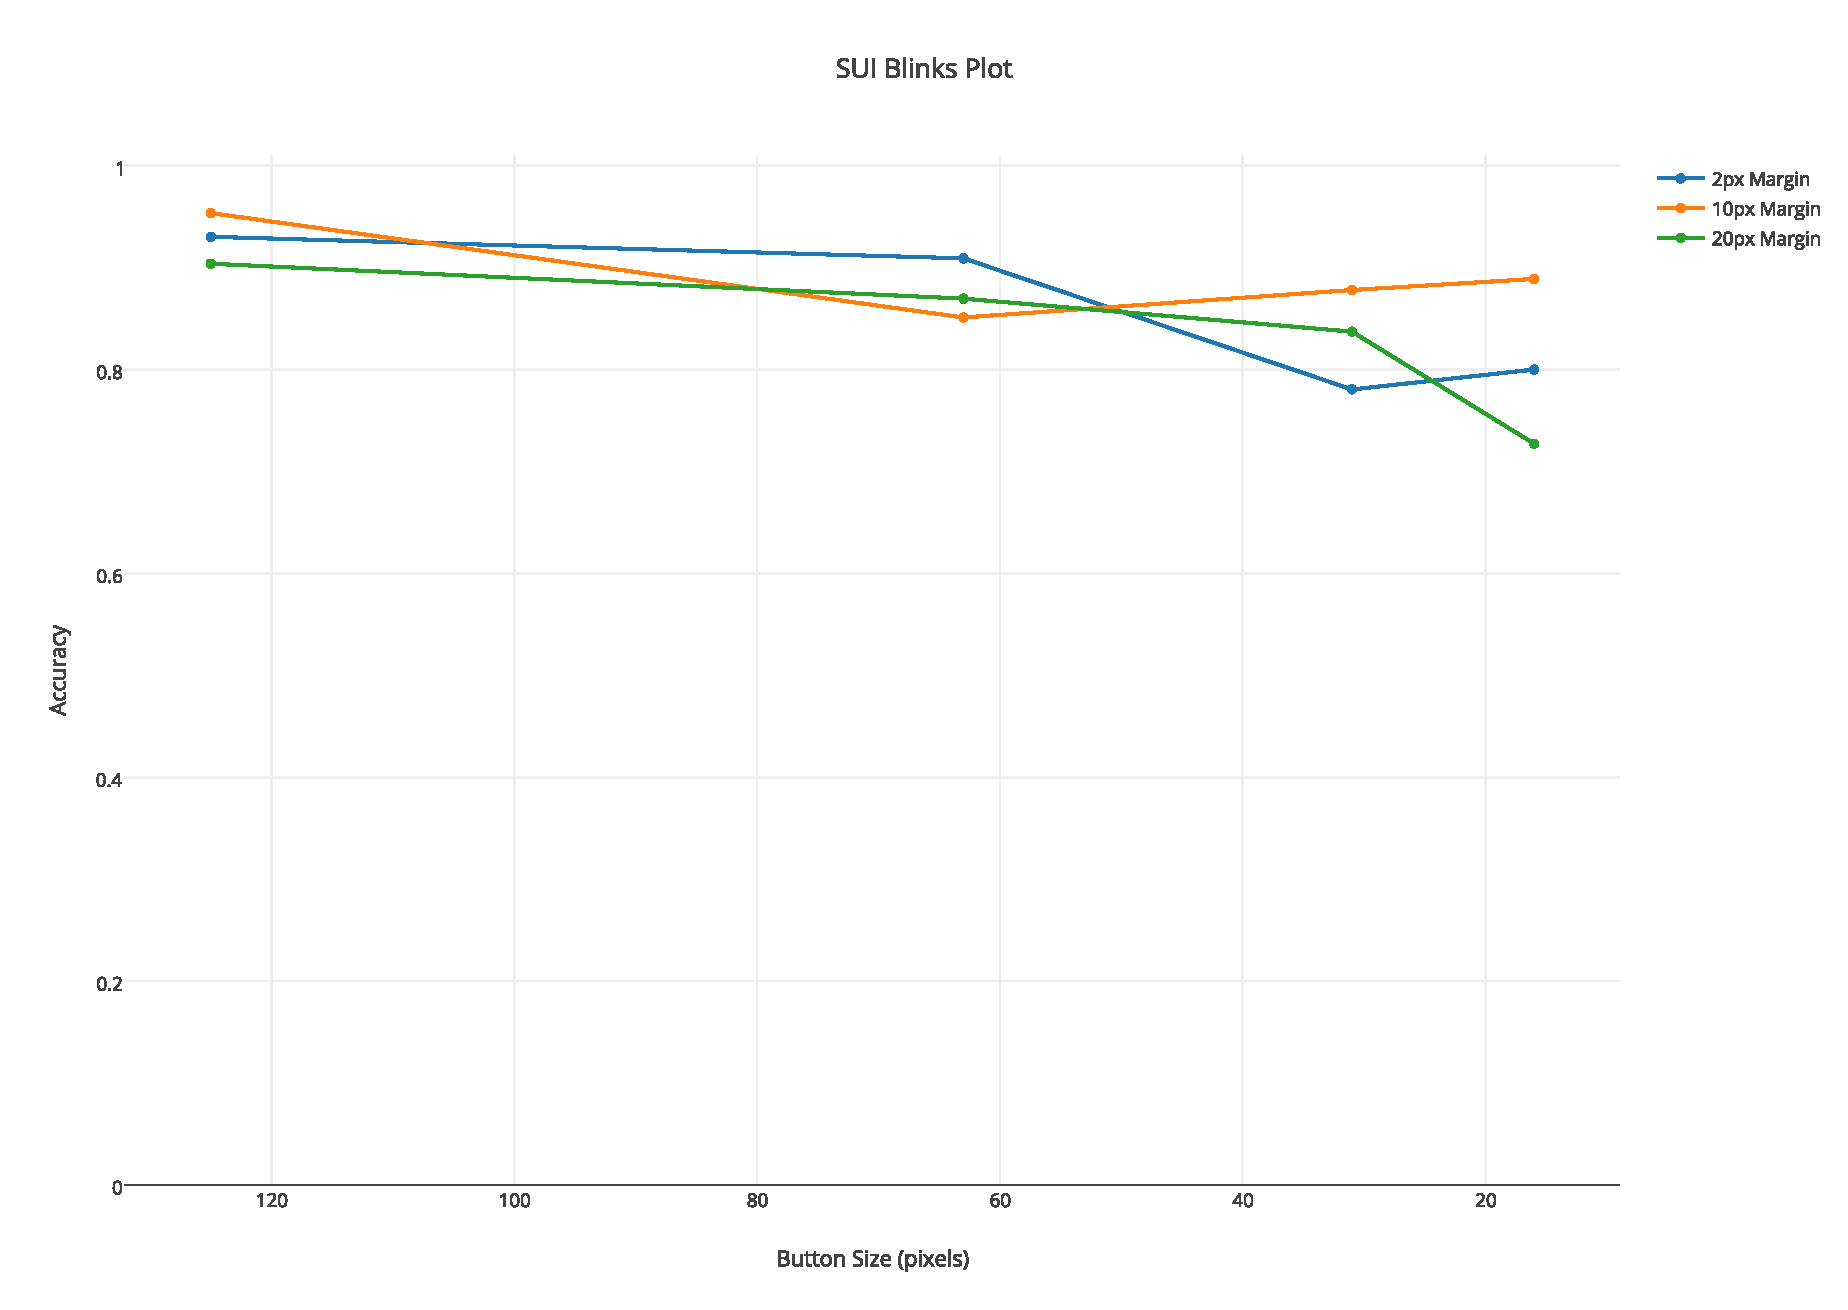
\includegraphics[width=0.9\columnwidth]{figures/blink-accuracy.pdf}
  \caption{Blink input modality accuracy with various margin and button sizes.
  }~\label{fig:blink-accuracy}
\end{figure}

\begin{figure}
\centering
  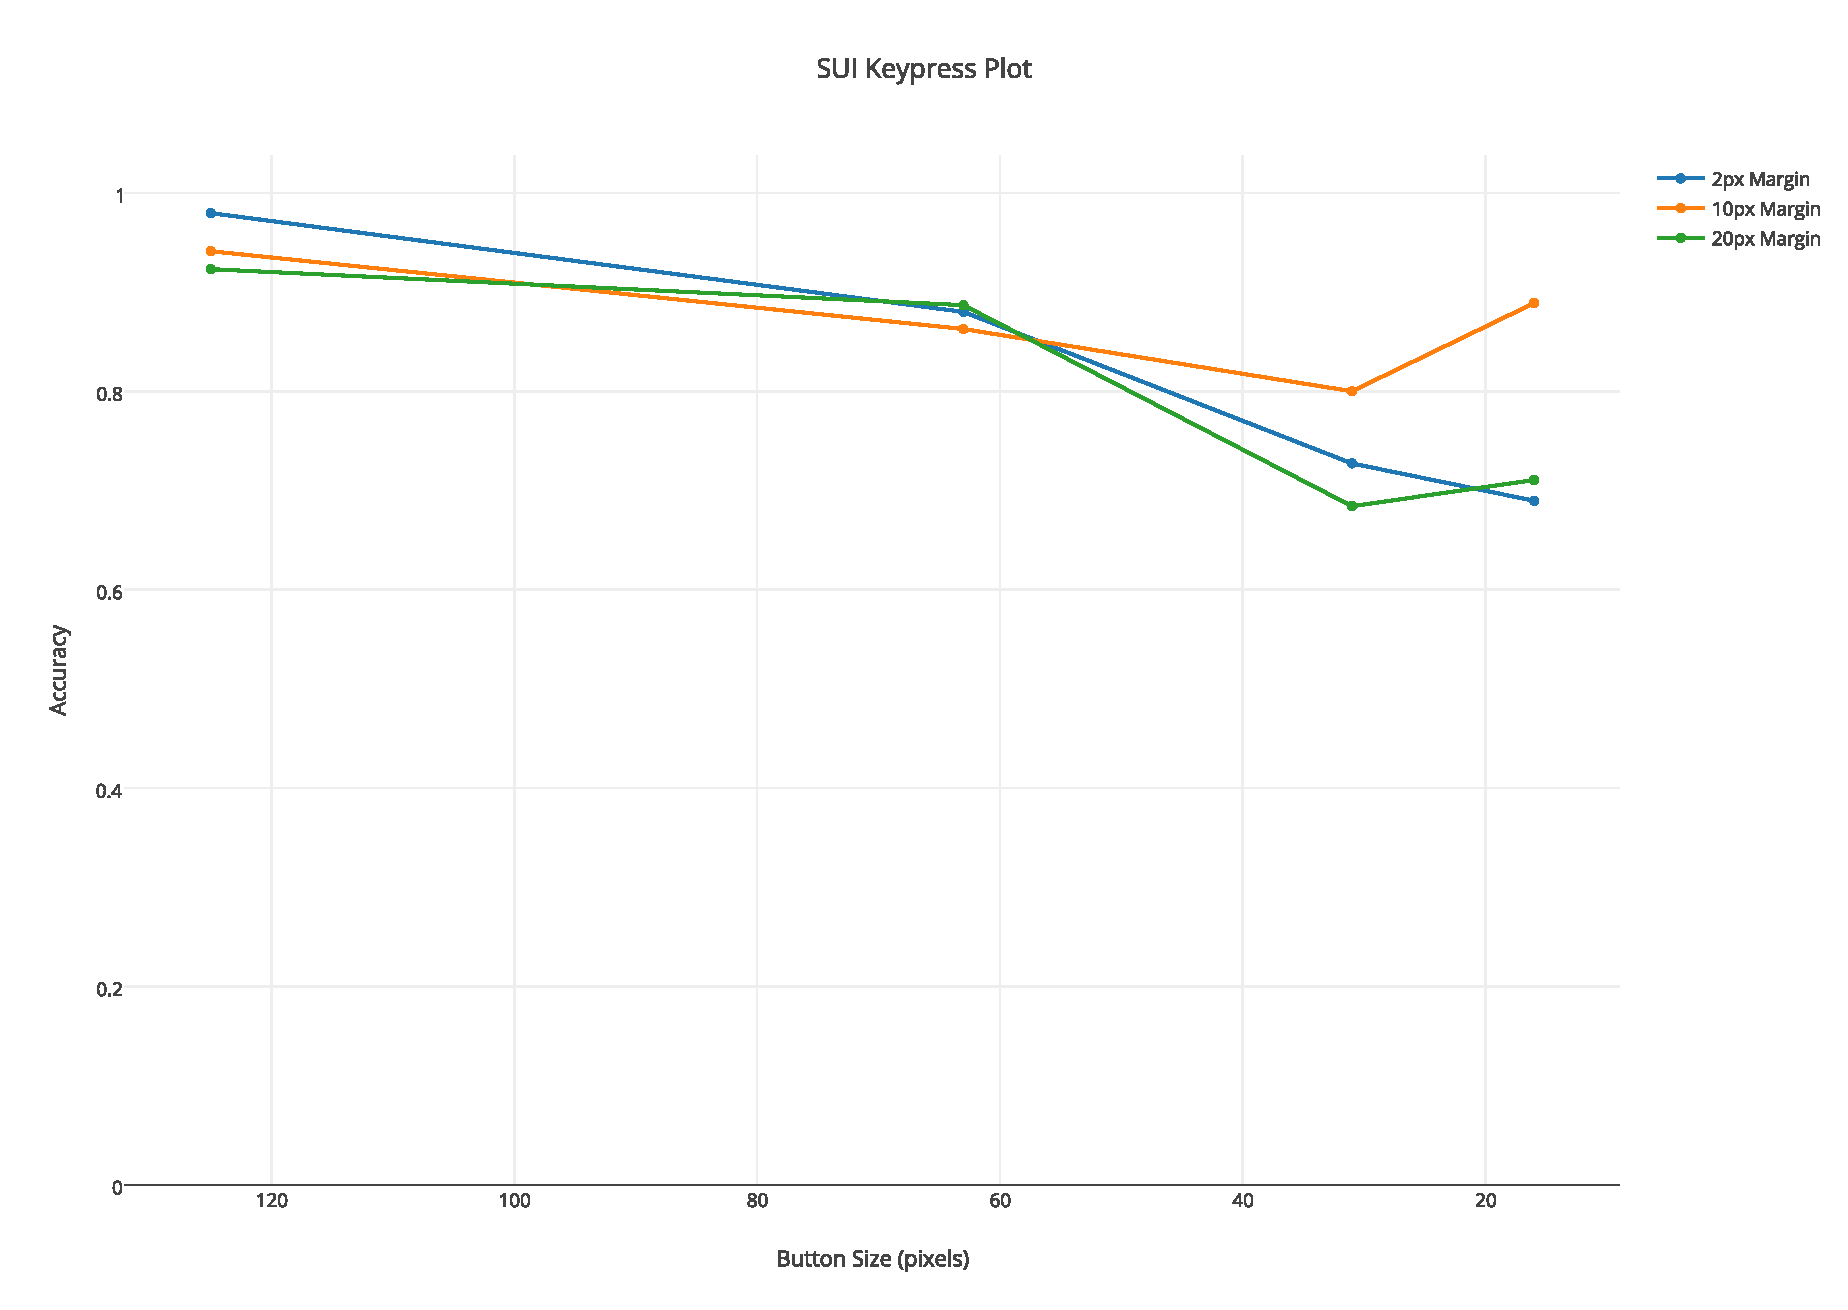
\includegraphics[width=0.9\columnwidth]{figures/keypress-accuracy.pdf}
  \caption{Keypress input modality accuracy with various margin and button sizes.
  }~\label{fig:keypress-accuracy}
\end{figure}

Figure \ref{fig:keypress-accuracy} shows an increase in accuracy at the smallest button size. This is due to the fact that not all users were able to complete the selection task (select a button) before the task timer ran out. \hl{Insert plot of the number of users who completed each input mode at each button size.}

\section{Discussion}


\subsection{Limitations}


\subsection{Recommendations}

\subsubsection{Element Density}

\subsubsection{Element Size}

\subsubsection{Eye Semantics}


\subsection{Future Work}

\subsubsection{Custom Calibration Interface}
The Eye Tribe tracker provides API access to calibration routines, so it is conceivable that in the future EyeJS could be extended to include a standardized user interface for calibrating the eye tracker.

\subsubsection{Continuous Calibration}
As eye trackers advance and presumably provide a more advanced interface for developers and applications, it could be possible to perform continuous calibration improvement of the eye-tracker by inferring interactions... activate some element therefore the user was probably looking at that element, therefore push a calibration offset point...



\section{Conclusion}



\section{Acknowledgments}



\balance{}

% REFERENCES FORMAT
\bibliographystyle{sigchi}
\bibliography{eyejs}

\end{document}

%%% Local Variables:
%%% mode: latex
%%% TeX-master: t
%%% End:
